\chapter{Mapping}

Mapping (or aligning) and assembly are the operations that allow us to make some sense out of fragments (input data) deriving from sequencing, produce assemblies. 

\begin{itemize}
    \item \textbf{Mapping} is a key step in a modern genomic analysis and consists in the process of aligning the reads on a reference genome, in order to assign them to a specific location. With mapping, insights like the expression level of genes can be gained.
    \item \textbf{Assembly} by contrast, is the process of aligning and merging overlapping sequences in longer consensus sequences in order to reconstruct the original sequence/genome.
\end{itemize}

A consensus sequence is  the calculated order of most frequent residues, either nucleotide or amino acid, found at each position in a sequence alignment
In many cases, someone may have already assembled the genome or part of the genome (available reference sequences), so we don't need to do sequence assembly, only mapping (like for the human genome). Assembly will be needed however when studying new organisms. 

Problems related to mapping and assembly: 

\begin{itemize}
    \item absence of DNA fragments covering the gaps, makes it difficult to order the contigs (since there is no connection)
    \item presence of DNA artefacts (those must be discriminated with Quality Control)
    \item repeated sequences
\end{itemize}

\section{Mapping}

The coverage, or read depth, is the average number of reads representing a given nucleotide in the reconstructed sequence (Some points of the reference sequence will be aligned with more reads, some with less. The average number of reads for each nucleotide is the coverage). 
The coverage of a genome is defined as the average coverage of each single nucleotide across all nucleotides of the genome. Additional info and examples at:  
% https://thesequencingcenter.com/knowledge-base/coverage/#:~:text=Coverage%20is%20defined%20as%20the,reference%20genome%20Escherichia%20coli%20BW2952.
A coverage of 1x does not mean that all reads are read once. This would be true if sampling were systematic, but sampling is not systematic, it is random and is biased. Hence, a coverage of 1x means that on average each nucleotide is covered once, but there will be some nucleotides covered more and some not covered (0 coverage). 
The coverage can be represented with a coverage map and can also be defined theoretically as:
Cov = (N * L)/G
where G is the length of the genome; N is the  number of reads; L is the average read length.
Knowing the wanted coverage is important to set up the machine in order to obtain the right number of reads (to achieve a certain coverage). A higher coverage means indeed more reads to be obtained. 

\subsubsection{Exercise on coverage}

\emph{How many reads do I need to cover the entire genome?}
Define the probability  to cover the full genome (with a certain epsilon subtracted - so not 100$\%$) or: define the number of reads N to cover the whole genome with a certain probability P = 1- epsilon.

\begin{figure}[h]
\centering
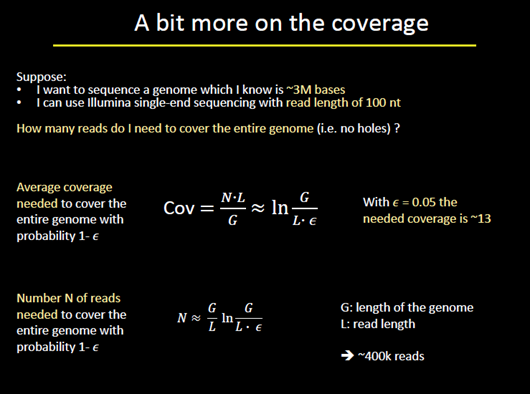
\includegraphics[width=0.6\textwidth]{coverage.png}
\caption{}
\end{figure}

In general, the sequence mapping process consists in performing comparisons between experimental sequence data (reads obtained with sequencing) with some reference information, like reference genomes and known genes (eg. the human genome). The comparison can lead to obtaining new information, such as the presence of SNPs which can be linked to pathological conditions or whatsoever, based on the starting point.

\begin{figure}[h]
\centering
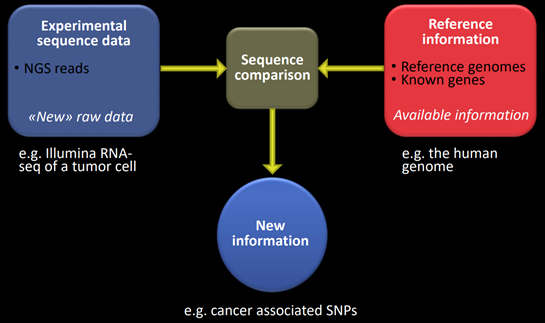
\includegraphics[width=0.6\textwidth]{SequenceComparison.png}
\caption{}
\end{figure}

\section{Mapping algorithm}

Over time many different mapping algorithms were implemented; some of them are not used anymore, while others are the base of current mapping and aligning genomic tools. 
Ideally, the \textbf{simplest aligning algorithm} could consists in:  
We have a smaller sequence that we want to align to a longer one. Start from the first position, align the query sequence against the subject, and look at how many nucleotides are correct (score: 4/10 = 40$\%$), then repeat for all positions until a perfect match is found (if found). The problem with this algorithm is that it doesn't consider insertions and deletions.

\subsection{Local vs Global alignment}
Sequence alignment can follow two different approaches.

\begin{enumerate}
    \item In \textbf{global alignment} an attempt is made to align completely the 2 sequences (end to end alignment). So global alignment finds the best alignment across the whole two sequences. This approach is suitable for comparing closely related sequences like homologous genes. 
    \item \textbf{Local alignment}, on the other hand, focuses on finding regions of similarity in parts of the sequences (so it aligns subsequences of the query sequence to a subsequence of the target sequence). This approach is suitable for aligning more divergent sequences or distantly related sequences. Used for example for finding out conserved patterns in DNA sequences of motifs in two proteins.
\end{enumerate}

Sequence similarity is connected with \textbf{evolutionary distance} (also for cell populations in a tumour). Very high similarity implies a very low distance. But when the similarity goes down and reaches the twilight zone, it is more difficult to define the evolutionary distance and to give meaning to results (the zone depends on the experiments).

\begin{figure}[h]
\centering
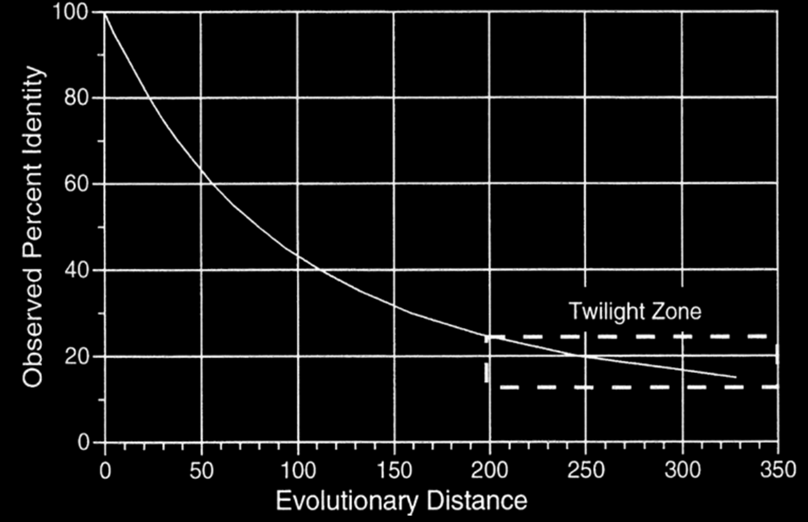
\includegraphics[width=0.6\textwidth]{EvolutionaryDistance.png}
\caption{}
\end{figure}

\subsection{Smith-Waterman algorithm  (local alignment) - 1981}

%Paper link: https://www.sciencedirect.com/science/article/abs/pii/0022283681900875?via%3Dihub
Take the algorithm for string recognition and apply it to find common molecular sequences. Not good for indels and substitutions. 
The S-W Algorithm is a local-alignment algorithm based on dynamic programming, whose aim is to find the best match among all possible (optimal local alignment) with respect to the scoring system used .
Firstly, we need to define a \textbf{score} for matches and penalties for mismatches and gaps (defined by the formula). 
The algorithm starts by putting zeros in the first row/column (\textbf{INITIALIZATION}). Then, starting from the first position H(1,1), at each iteration a number, based on the formula, is added (\textbf{ITERATION}). The number to be added is the greater between the 4 numbers defined by the formula, where d represents the penalty for gaps, and  s(x,y) = score when 2 NTs are the same (This gives a score of 5 if the 2 bases are equal, -3 if they are different) (PARAMETER SETTING).

\begin{figure}[h]
\centering
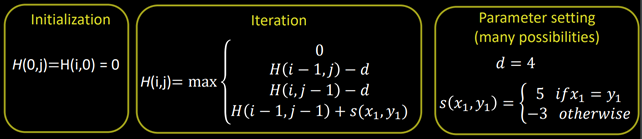
\includegraphics[width=0.6\textwidth]{Waterman.png}
\caption{}
\end{figure}

\textbf{Example}

First position H(1,1) = (G,C), max between: 

\begin{itemize}
    \item 0
    \item H(i-1, j) = 0-4 = -4
    \item H(i, j-1) = 0-4 = -4
    \item H(diag) + s(x, y) = 0 – 3 = -3
    \item $\xrightarrow[]{}$ We put 0
\end{itemize}

Second position H(2,1) = (A, G):

\begin{itemize}
    \item - 0
    \item -4
    \item -4
    \item -3
    \item $\xrightarrow[]{}$ We put 0
\end{itemize}

Third position H(3,1) = (C e C):

\begin{itemize}
    \item - 0
    \item -4
    \item -4
    \item 0 + 5 (since C=C)
    \item $\xrightarrow[]{}$ We put 5 
\end{itemize}

Here we also put an arrow indicating the nucleotide in the diagonal, to indicate that the 5 score derived from that point (hence from that path).  The arrows are needed to reconstruct the alignment at the end of the process. The iteration is performed for each cell of the table (column wise).
The parameters chosen for d (gap penalty) and s(x,y) (match or mismatch) can change the results. 
Final Solution: 

\begin{figure}[h]
\centering
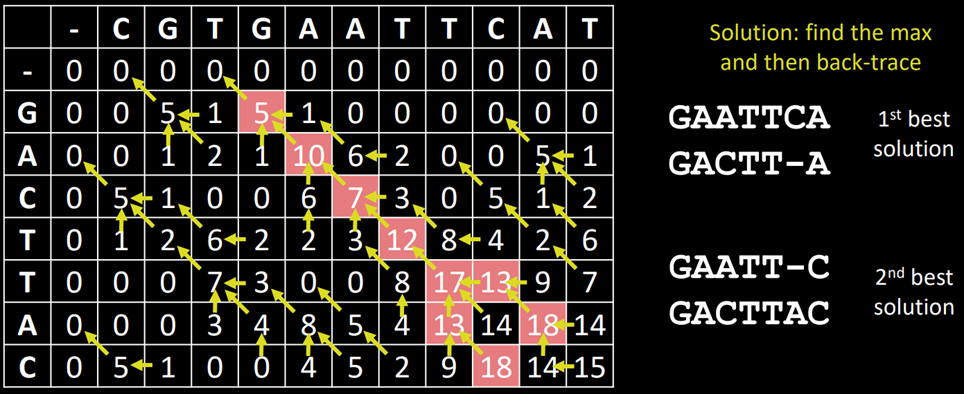
\includegraphics[width=0.6\textwidth]{Aligning.png}
\caption{Aligning CGTGAATTCAT and GACTTAC}
\end{figure}

Find the \textbf{maximum number} (18, here we have 2 of them) and go back following the arrows. In case of multiple highest scores, traceback should be done starting with each highest score.
From this path, the sequence is constructed by these rules:

\begin{itemize}
    \item A diagonal arrow represents a match or mismatch, so the letter of the column and the letter of the row of the origin cell will align.
    \item A horizontal or vertical arrow represents an indel. Vertical arrows will align a gap ("-") to the letter of the row (the "side" sequence), horizontal arrows will align a gap to the letter of the column (the "top" sequence).
    \item If there are multiple arrows to choose from, they represent a branching of the alignments. If two or more branches all belong to paths from the bottom right to the top left cell, they are equally viable alignments. In this case, note the paths as separate alignment candidates.
\end{itemize}

This algorithm is not used anymore due to a too high computational expense (huge number of comparisons for real genomes) and storage (memory and speed). In fact comparing two Eukaryotic genomes will result in a excessively great aligning matrix ($\sim$3Gb x $\sim$3Gb), and also using small reads against the human genome is unfeasible: 100 x $\sim$3Gb for each read!

\subsection{Needleman-Wunsch algorithm (global alignment)}

This global alignment algorithm was developed in 1970 and is also based on dynamic programming. The purpose of the algorithm is to find all possible alignments having the highest score. Again, a scoring system must be defined, then the algorithm proceeds in a similar way as the SW. 

\begin{figure}[h]
\centering
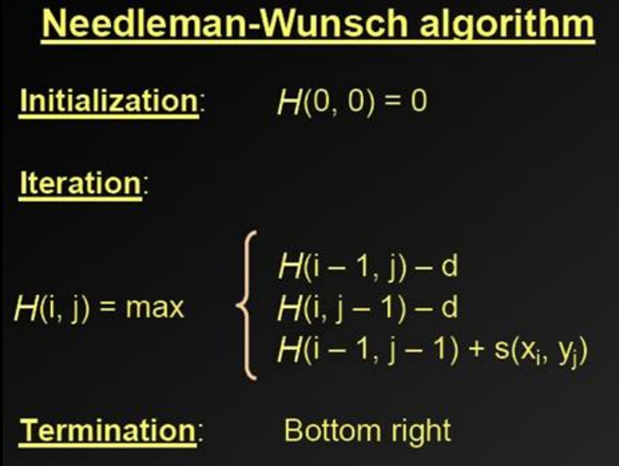
\includegraphics[width=0.6\textwidth]{Needleman.png}
\caption{}
\end{figure}

The differences are:

\begin{itemize}
    \item Initialization: we start from only one value, one zero, putted in H(0,0) (need to start from the first nucleotide - global). 
    \item The formula contains no 0 anymore, it adds the maximum score between 3 possible scores, we are always comparing with the first nucleotide of the sequence. 
\end{itemize}

\begin{figure}[h]
\centering
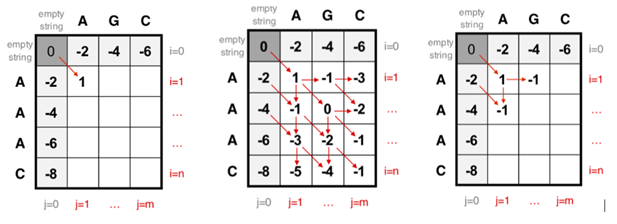
\includegraphics[width=0.6\textwidth]{Needleman2.png}
\caption{}
\end{figure}

New algorithms were implemented later. 
BWA and BowTie2 are the best ones available right now for short reads. Blast could go too but it would take a lot of time. 

\begin{figure}[h]
\centering
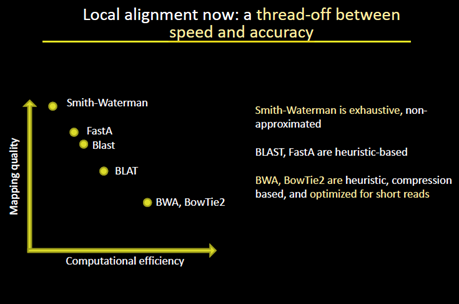
\includegraphics[width=0.6\textwidth]{LocalAlignment.png}
\caption{}
\end{figure}

The methods going from FastA to BowTie2 are \textbf{heuristic methods}: the solution found does not need to be the best one, but the best approximation given certain parameters (like time). Also, Blast gives an answer based on a fixed level of sequence similarity (in a reasonable amount of time) and gives no result under that level. So Blast online is not very sensitive, it is trained to provide only very good results to not overload the servers. 
A \textbf{heuristic}, or heuristic technique, is any approach to problem solving or self-discovery that employs a practical method that is not guaranteed to be optimal, perfect, or rational, but is nevertheless sufficient for reaching an immediate, short-term goal or approximation. Where finding an optimal solution is impossible or impractical, heuristic methods can be used to speed up the process of finding a satisfactory solution. Heuristics can be mental shortcuts that ease the cognitive load of making a decision.
BWA and BowTie2 are also ‘compression based’ algorithms, meaning that they exploit data compression techniques in order to compress reference genome files to reduce the number of bits used to encode the document (better explained below).

\subsection{BLAST (Basic Local Alignment Search Tool)}

%Tutorial: https://www.youtube.com/watch?v=HXEpBnUbAMo&ab_channel=JHUAdvancedAcademicPrograms
Despite its limitations, Blast is still used a lot and when it was first released it revolutionised the field making sequence alignment available for anyone and for any computer (it can be run online).
How does it work? Steps:

\begin{enumerate}
    \item \textbf{Seeding}: find perfect or almost exact k-mer matches (series of sequences with defined length). The idea is to look for identical short matches and try to expand from that. 
    \item \textbf{Extension}: extend the seeds at point one 1 with possibly some non-exact but high-score matches, that permit to obtain better alignments.
    \item \textbf{Evaluation}: create alignments for the regions of high-scoring extended seeds. Every time the statistical significance of the match is evaluated with methods inspired on the NW and SW approaches.  
\end{enumerate}

In online Blast tools the seed is set to 25/29. If a sequence of that length does not match perfectly another sequence we will have no results. One solution would be to lower the seed, but this cannot be done online because it would take too much time. Another option is to reduce the dataset in which we search.
There are many types of blast available, shown in figure:

\begin{figure}[h]
\centering
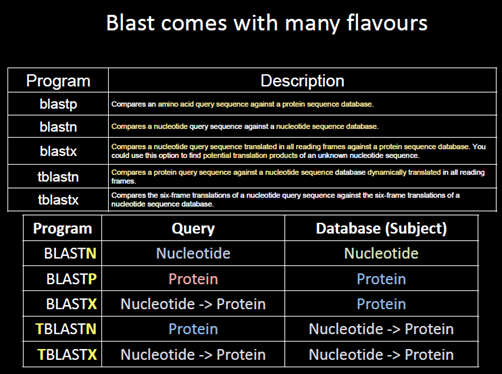
\includegraphics[width=0.6\textwidth]{Blast.png}
\caption{}
\end{figure}

\textbf{Scoring matrices} are very important especially for amino acids, they are used to score alignments between protein sequences. Blosum 62 (BLOcks SUbstitution Matrix) is one of the most used.
They put non simple penalties in substitutions of different amino acids, for example based on the functional properties of the substitutions. A scoring matrix contains values proportional to the probability that amino acid i mutates into amino acid j for all pairs of amino acids. Such matrices are constructed by assembling a large and diverse sample of verified pairwise alignments of protein sequences.
Other \textbf{parameters} can be set in online BLAST:

\begin{itemize}
    \item Max target sequences $\xrightarrow[]{}$ number of reported sequences 
    \item Expected threshold $\xrightarrow[]{}$ e-value
    \item Words size $\xrightarrow[]{}$ seed
    \item Gap cost $\xrightarrow[]{}$ cost for adding multiple gaps. Linear = twice the gap penalty (if I have to add a second gap after another one).
    \item Filter low complexity regions to avoid getting stuck 
\end{itemize}

\subsubsection{BLAST E-value}

If we have a match and the database is random, how many other matches I will likely find?

\begin{figure}[h]
\centering
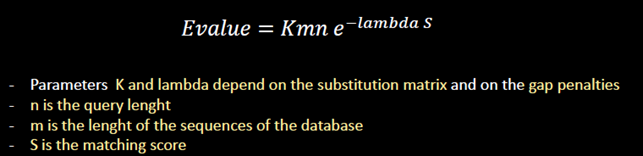
\includegraphics[width=0.6\textwidth]{Evalue.png}
\caption{}
\end{figure}

The \emph{e-value} represents the number of distinct alignments with a score equivalent to or higher than S, that are expected to occur in a database search by chance. An e-value of 10 means that up to 10 alignmentscan be expected to be found just by chance, given the same size of a random database. E-value can be used as a first quality filter for the BLAST search result, to obtain only results equal to or better than the number given by the e-value option. Blast results are sorted by E-value by default (best hit in first line).
The smaller the e-value, the better is the match. A small e-value means a low number of hits, but of high quality, whereas a high e-value indicates many hits, partly of low quality (if the number of better possible alignments is high, it means that it is particularly probable to find by chance an alignment which is better the the one found, and so it is more probable that those alignments are bad). 
There is a relationship between the E-value and the p-value. 

\begin{itemize}
    \item The E-value is the number of sequences that we would find by chance;
    \item The p-value measures the probability of finding by chance another sequence with an equal or better score.
\end{itemize}

%aggiungi formula

\subsection{Speed seed alignment}

There are algorithms implemented 10/15 years ago that focus on seeds -> not used anymore. 
Those methods cut both the reads and the reference sequence (read-sized pieces of reference sequence) into small seeds. The reference seeds are then stored in an index (hash look-up table).
The idea is to do that for all possible k-mers. Eg. we choose a seed of 10: the first starts at position 1, the second at position 2, ecc. And then to look up seeds for each read and identify the positions in genome where spaced seed pair is found. 

\begin{itemize}
    \item 1 SNPs means that at most 1 seed is not-matching.
    \item X SNPs means that at most X seeds are not-matching.
\end{itemize}

Algorithms based on this approach are: Maq, SOAP, MOSAIK. 
Problem: the lookup table (the reference) for the human genome is too big: 50Gb $\xrightarrow[]{}$ problem in RAM.

\subsection{Burrow-Wheeler alignment}
This algorithm is based on a very efficient way to store the reference genome, based on the BW transformation, that allows to have a reference index which is way lighter (with respect to the spaced seed approach); in fact, at the end of the transformations, equal letters are next to each other. It is successful because the database is compressed and does not need to be decompressed. However, when we compress a file, the compression must be reversible. There must be a way to go from the BW compressed/transformed index to the original one, to find reads in the genome. 
The search is based on finding suffixes of the reads in the BW structure. With this approach the index of the human genome is around 2GB. The algorithms BW-based are the fastest currently available. 
BWT is also used in text compression.
Example:
We want to compress the word BANANA
\begin{itemize}
    \item - we take all the rotations of the word
    \item we sort them based on lexigographic order (Lex order - lexicographical order is a generalization of the alphabetical order of the dictionaries to sequences of ordered symbols) 
    \item we take the last column
\end{itemize}

We end up with a string which is more compressible, there are sequences of the same letters that can be described at a higher level (Eg. there is 1 B, 2 NN, ecc)
In the method shown, in order to \textbf{reverse the transformation} and go back to the original word, the input sequence (output of the compression) is added as a column and then sorted (based in lex order), and this two passages are repeated as many times as are the characters of the sequence (8 in this case), obtaining at the end a matrix with equal number of columns and rows. As a result we go back to the ordered sequence of the word's rotations, in which the last one (last line) is the original input string. 
It takes a lot of time but it makes it reversible; plus, there are actually smarter ways to go back, such as ones base on the LF property.

\subsection{LF (Last-First) property}

As in the previous method, the first step consists in sorting all word's rotations and taking the last column which will be the compressible one.
The LF property is then applied to the list of all rotations,
to get back to the input sequence, by following this principle: the ith occurrence of character X in the last column corresponds to the same text character as the ith occurrence of X in the last column.
Example: We want to reverse the transformation of the string "gc$\$$aaac”. 

\begin{figure}[h]
\centering
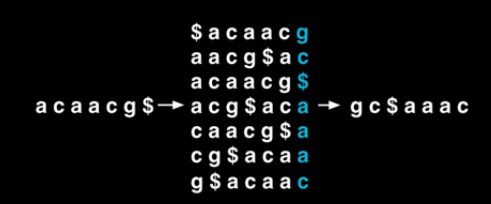
\includegraphics[width=0.6\textwidth]{1LF.png}
\caption{}
\end{figure}

\begin{figure}[h]
\centering
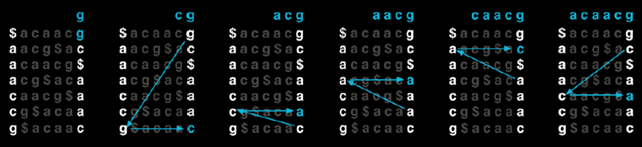
\includegraphics[width=0.6\textwidth]{2LF.png}
\caption{}
\end{figure}

\begin{itemize}
    \item \emph{g} is the first occurrence of g in the last column and corresponds to (arrow) the first occurrence of \emph{g} in the first column. Tracing a horizontal arrow gives the next nucleotide.
    \item \emph{c} is the second occurrence in the second column and corresponds to (arrow) the second occurrence of \emph{c} in the first column. Tracing an horizontal arrow gives the next nucleotide.
    \item \emph{a} is the third occurrence of a in the second column and corresponds (arrow) to the third occurrence of \emph{a} in the first column. Tracing an horizontal arrow gives the next nucleotide.
\end{itemize}

And so on. Each time we keep track of the character that we are looking at and we end up by constructing the original word. With this method we reconstruct the word from its end to its beginning (backward). 

\subsection{Exact mapping using LF property}

In mapping, we can look for sequence matches using the compressed database.
Backward exact mapping works by calculating the range of matrix rows beginning with successively longer suffixes of the query.
Example: we want to match the string 'aac' with the database.

\begin{figure}[h]
\centering
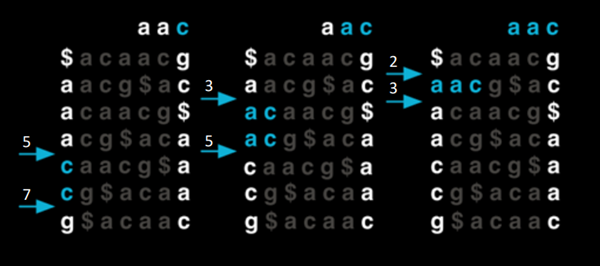
\includegraphics[width=0.6\textwidth]{3LF.png}
\caption{}
\end{figure}

\begin{itemize}
    \item we take the 'first suffix' \textbf{c} of the query string and we look for it in the first column. We find 2 matches in lines 5 and 6, so in the range 5-7.
    \item we pass to a 'second longer suffix' \textbf{ac} and see if we can find it in the matrix $\xrightarrow[]{}$ lines 3 and 4, range 3-5.
    \item we look at the suffix \textbf{aac} and find it in the 2-3 range.
\end{itemize}

Doing the backward matching we exploit the characteristics of the BWT transform. This same approach could be used to find a match between a query read and a reference genome which has been compressed using the BW alignment.
The problem is that it does not take into accounts indels, mismatches. 
A possible solution to this problem could be the \textbf{inexact mapping}. 
Perform exact mapping and, if the query is not found, go back and perform backtracking by hypothesising mismatches. For example we want to find a match for the query GGTA. As always, we start looking for a match starting from the last character.

\begin{itemize}
    \item we find a match for a, t, g but not for the last g. 
    \item so we go back and hypothesize a mismatch for the first letter a. We then look for all the matches that we could find if we replace a with another nucleotide (we do the same for the other NTs in the query?). 
    \item we find than by replacing a with a g, we find a match (ggtg) (not exact match).
\end{itemize}

The Burrows-Wheeler algorithm is used in BowTie and Bowtie2. 
Right now there are many algorithms to choose between and many review papers compare their characteristics and performance. No tool outperforms the others in all the test, hence the decision of which algorithm to choose must depends on the specific needs. 

\begin{figure}[h]
\centering
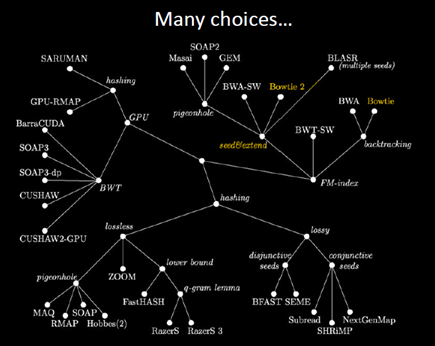
\includegraphics[width=0.6\textwidth]{Choices.png}
\caption{}
\end{figure}
